\chapter{Decodifica} \label{chap:decodifica}
	
	Lo schema generale della decodifica di un file \texttt{.mp3} è rappresentato in Figura \ref{fig:decode_layout}. In linea di massima, vengono ripercorse le fasi descritte nel Capitolo \ref{chap:codifica}, ma al contrario
	
	\begin{figure}[h!]
		\centering
			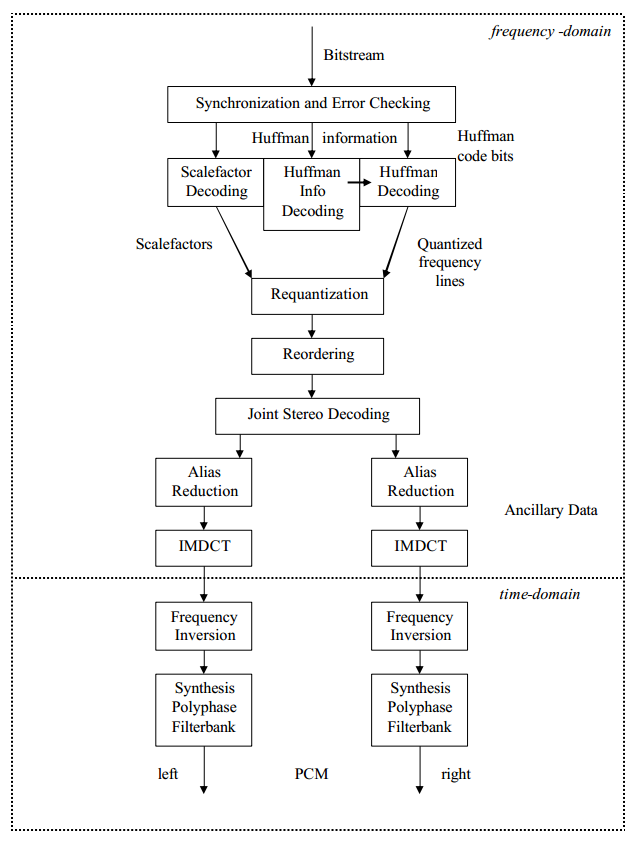
\includegraphics[scale=1]{decode_layout.png}
		\caption{Schema della decodifica MP3.}
		\label{fig:decode_layout}
	\end{figure}
	
	\section{Sincronizzazione} \label{sec:sincronizzazione}
		
		Il flusso di bit letti dal file \texttt{.mp3} viene scorso finhé non viene trovata la word di sincronizzazione (12 bit a 1). Se non viene rilevata la word di sincronizzazione di un frame, i dati non possono essere codificati ed il file è corrotto.
		
	\section{Decodifica Huffman e dei parametri relativi} \label{sec:decodifica_huffman}
		
		Innanzitutto è necessario decodificare i sample quantizzati tramite decodifica Huffman. Abbiamo visto che la codifica di Huffman è una codifica a lunghezza variabile ed inoltre dipende dalla tabella di Huffman impegata. Ad esempio non è possibile prendere una serie di bit a caso e sperare di decodificarli: è necessario leggere le sequenze codificate dall'inizio e sapere come sono stati codificati i dati. Vengono quindi decodificati (dalla Side Information) tutta una serie di parametri relativi alla codifica Huffman, come la suddivisione in regioni e sottoregioni, le tabelle di Huffman utilizzate, ecc \dots.\\
		Una volta in possesso di tutti i parametri necessari, i 576 sample verranno decodificati, utilizzando le tabelle di Huffman. Si noti che nel caso in cui meno di 576 sample siano trovati, dovranno essere inseriti i sample mancanti come sequenze di zeri.
		
	\section{Decodifica dei fattori di scala} \label{sec:decodifica_fattori_scala}
		
		In questa fase vengono decodificati i fattori di scala, che si trovano all'inizio dei dati principali di ogni granulo. I dati relativi a dove trovare i fattori di scala sono codificati nella Side Information di ogni granulo.
		
	\section{Riquantizzazione} \label{sec:riquantizzazione}
		
		Ricavando i valori di campi come global\_gain o scalefac\_scale si possono riquantizzare i sample quantizzati e scalati ottenuti dalla decodifica di Huffman, ottenendo le linee di frequenza generate dall'MDCT. I dati sui fattori di scala, necessari per la riquantizzazione, vengono forniti dallo step precedente (decodifica dei fattori di scala). Si osservi che in questo step vengono utilizzate funzioni di riquantizzazione differenti a seconda della finestra usata.
		
	\section{Riordinamento} \label{sec:riordinamento}
		
		Le linee di frequenza generate dal processo di riquantizzazione non sono sempre nell'ordine in cui dovrebbero essere dopo l'MDCT. Infatti se nell'MDCT era stata usata una finestra lunga, allora le linee di frequenza erano ordinate prima per sottobanda e poi per frequenza, mentre se erano state usate finestre corte erano ordinate per sottobanda, per finestra e quindi per frequenza. Tuttavia per aumentare l'efficienza della codifica Huffman, le linee di frequenza relative a finestre corte venivano riordinate, prima per sottobanda, poi per frequenza ed infine per finestra, in quanto sample di frequenza vicina hanno molto probabilmente un valore simile.\\
		Vengono allora cercate le linee di frequenza relative alle finestre corte in tutte le sottobande e, quando trovate, vengono riordinate, in modo da avere esattamente l'output dell'MDCT in fase di codifica.
		
	\section{Decodifica stereo} \label{sec:decodifica_stereo}
		
		Questo passaggio serve per separare l'insieme di sample generato in due segnali distinti: destro e sinistro. Per ricavare la modalità di canale utilizzata si leggo i valori dei campi Mode e Mode Extension dall'header del frame.
		
	\section{Riduzione dell'aliasing} \label{sec:riduzione_aliasing}
		
		Prima di invertire l'MDCT è necessario ridurre l'aliasing prodotto dal banco filtri di analisi. Questo viene fatto applicando una serie di 8 \textit{calcoli a farfalla} (si veda la Figura \ref{fig:butterfly}) per ogni sottobanda, che rimuovono gli artefatti dal segnale.
		
		\begin{figure}[h!]
			\centering
				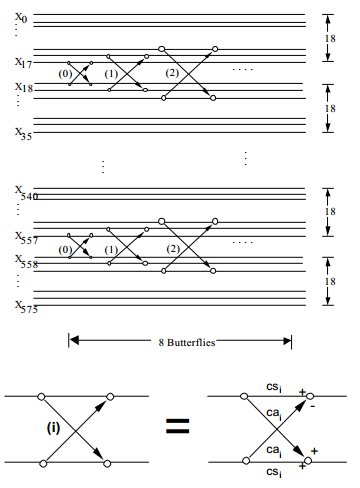
\includegraphics[scale=1]{butterfly.png}
			\caption{Riduzione dell'aliasing tramite calcoli a farfalla.}
			\label{fig:butterfly}
		\end{figure}
		
	\section{IMDCT} \label{sec:imdct}
		
		A questo punto è possibile applicare una \textit{IMDCT}, ovvero una \textit{Trasformata Discreta del Coseno Modificata Inversa}. L'IMDCT prende in input 576 linee di frequenza e restituisce 576 sample a dominio di tempo, suddivisi in 32 sottobande (18 sample per sottobanda).\\
		\\
		Analogamente alla (\ref{eqn:mdct}), la formula dell'IMDCT è la seguente:
		
		\begin{equation} \label{eqn:imdct}
			y_n = \frac{1}{N} \sum_{k=0}^{N-1}x_k\cdot\cos\left[\frac{\pi}{N}\left(n+\frac{1}{2}+\frac{N}{2}\right)\left(k+\frac{1}{2}\right)\right], \qquad n=0,\dots,2N-1.
		\end{equation}
		
	\section{Inversione di frequenza} \label{sec:inversione_frequenza}
		
		Dal momento che il banco filtri di analisi polifasico ha invertito le frequenze (similmente a quanto accade con la Trasformata di Fourier e sue derivate), per compensare si moltiplica ogni sample di indice dispari di ogni sottobanda dispari per $-1$.
		
	\section{Banco filtri di sintesi polifasico} \label{sec:banco_filtri_sintesi_polifasico}
		
		Infine, vengono fatti passare i sample di ogni sottobanda da un banco filtri di sintesi polifasico, che rappresenta l'inverso del banco filtri di analisi polifasico, visto in fase di codifica. Il risultato sono 576 sample PCM, per canale, che corrispondono al segnale audio decodificato.